

\chapter*{A - Github repository}
\addcontentsline{toc}{chapter}{\protect\numberline{}A - Github repository} 

All code and latex-files used in this document are included in the Github repository linked below. Further explanations are given in the readme-file. 


\subsection*{Github repository link}
\begin{itemize}
    \item \url{https://github.com/ninasalvesen/thesis_latex_template}
\end{itemize}


%%%%%%%%%%%%%%%%%%%%%%%%%%%%%%%%%%%%%%%%%%%%%%%%%%%%%%%%


\chapter*{B - Sidenote statistics}
\addcontentsline{toc}{chapter}{\protect\numberline{}B - Sidenote statistics} 

%For included tables and figures renew the numbering such that they are numbered by the appendix they are attached to and not to the conclusion chapter
\renewcommand{\thefigure}{B.\arabic{figure}}
\setcounter{figure}{0}
\renewcommand{\thetable}{B.\arabic{table}}
\setcounter{table}{0}


\section*{\large{B1 - Some random table}}
\vspace*{1cm}

Remember to only include one thing per page in the appendices.

\begin{table}[ht!]
\centering
    \begin{tabular}{ m{4cm} m{2.5cm} m{2.5cm} m{2.5cm} } 
    \toprule
    \toprule
    \textbf{Statistic} & \textbf{One} & \textbf{Two}  \\
    \midrule
    Count   & 387317    & 283960    \\[1.3ex]
    Mean    & 130.66    & 134.18    \\[1.3ex]
    Std     & 248.09    & 230.32    \\[1.3ex]
    Q1      & 31.00     & 21.00     \\[1.3ex]
    Median  & 67.00     & 63.00     \\[1.3ex]
    Q3      & 142.00    & 159.00    \\[1.3ex]
    Min     & 0.00      & 0.00      \\[1.3ex]
    Max     & 14519.00  & 14253.00  \\[1.3ex]
    \bottomrule
    \bottomrule
    \end{tabular}
\caption[Statistics on something]{Table of statistics on some sidenote data.}
\end{table}


% Page without title but section title:
\newpage
\section*{\large{B2 - Some other random table}}
\vspace*{1cm}

\begin{table}[ht!]
\centering
    \begin{tabular}{ m{4cm} m{2.5cm} m{2.5cm} m{2.5cm} } 
    \toprule
    \toprule
    \textbf{Statistic} & \textbf{Three} & \textbf{Four}  \\
    \midrule
    Count   & 387317    & 283960    \\[1.3ex]
    Mean    & 130.66    & 134.18    \\[1.3ex]
    Std     & 248.09    & 230.32    \\[1.3ex]
    Q1      & 31.00     & 21.00     \\[1.3ex]
    Median  & 67.00     & 63.00     \\[1.3ex]
    Q3      & 142.00    & 159.00    \\[1.3ex]
    Min     & 0.00      & 0.00      \\[1.3ex]
    Max     & 14519.00  & 14253.00  \\[1.3ex]
    \bottomrule
    \bottomrule
    \end{tabular}
\caption[Statistics on something else]{Table of statistics on some other sidenote data.}
\end{table}



\newpage
\section*{\large{B3 - Some random figure}}
\vspace*{1cm}

\begin{figure}[H]
  \centering
  \subfloat[Data set sizes for data X.]
  {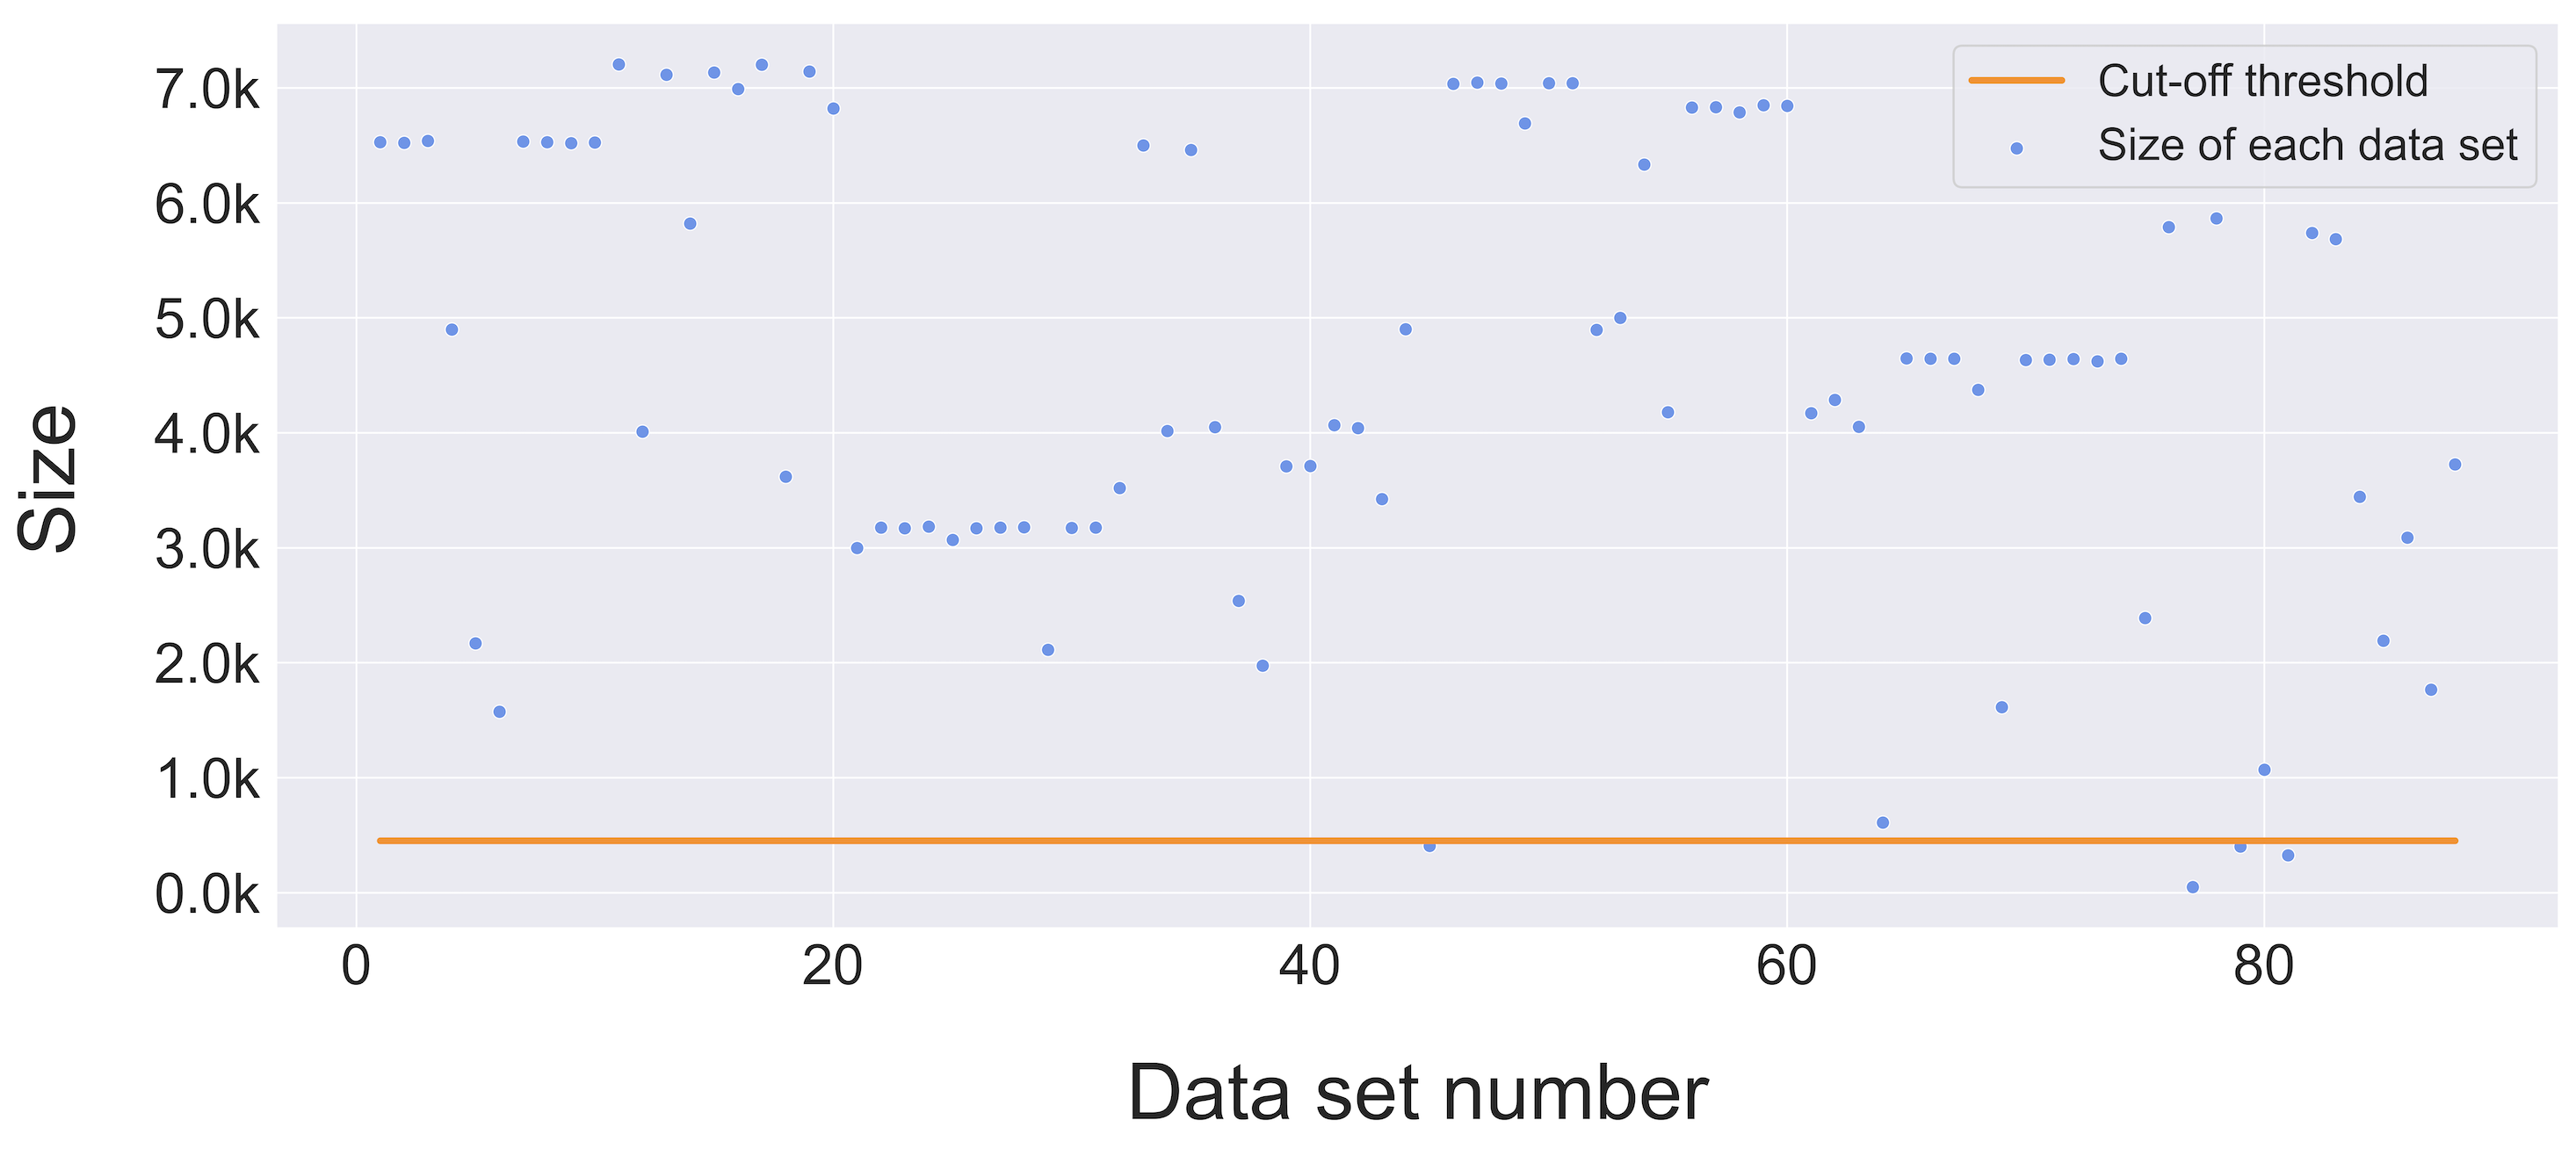
\includegraphics[width=1\textwidth]{Figures/dataset_X.png}}
  \hfill
  \subfloat[Data set sizes for data Y.]
  {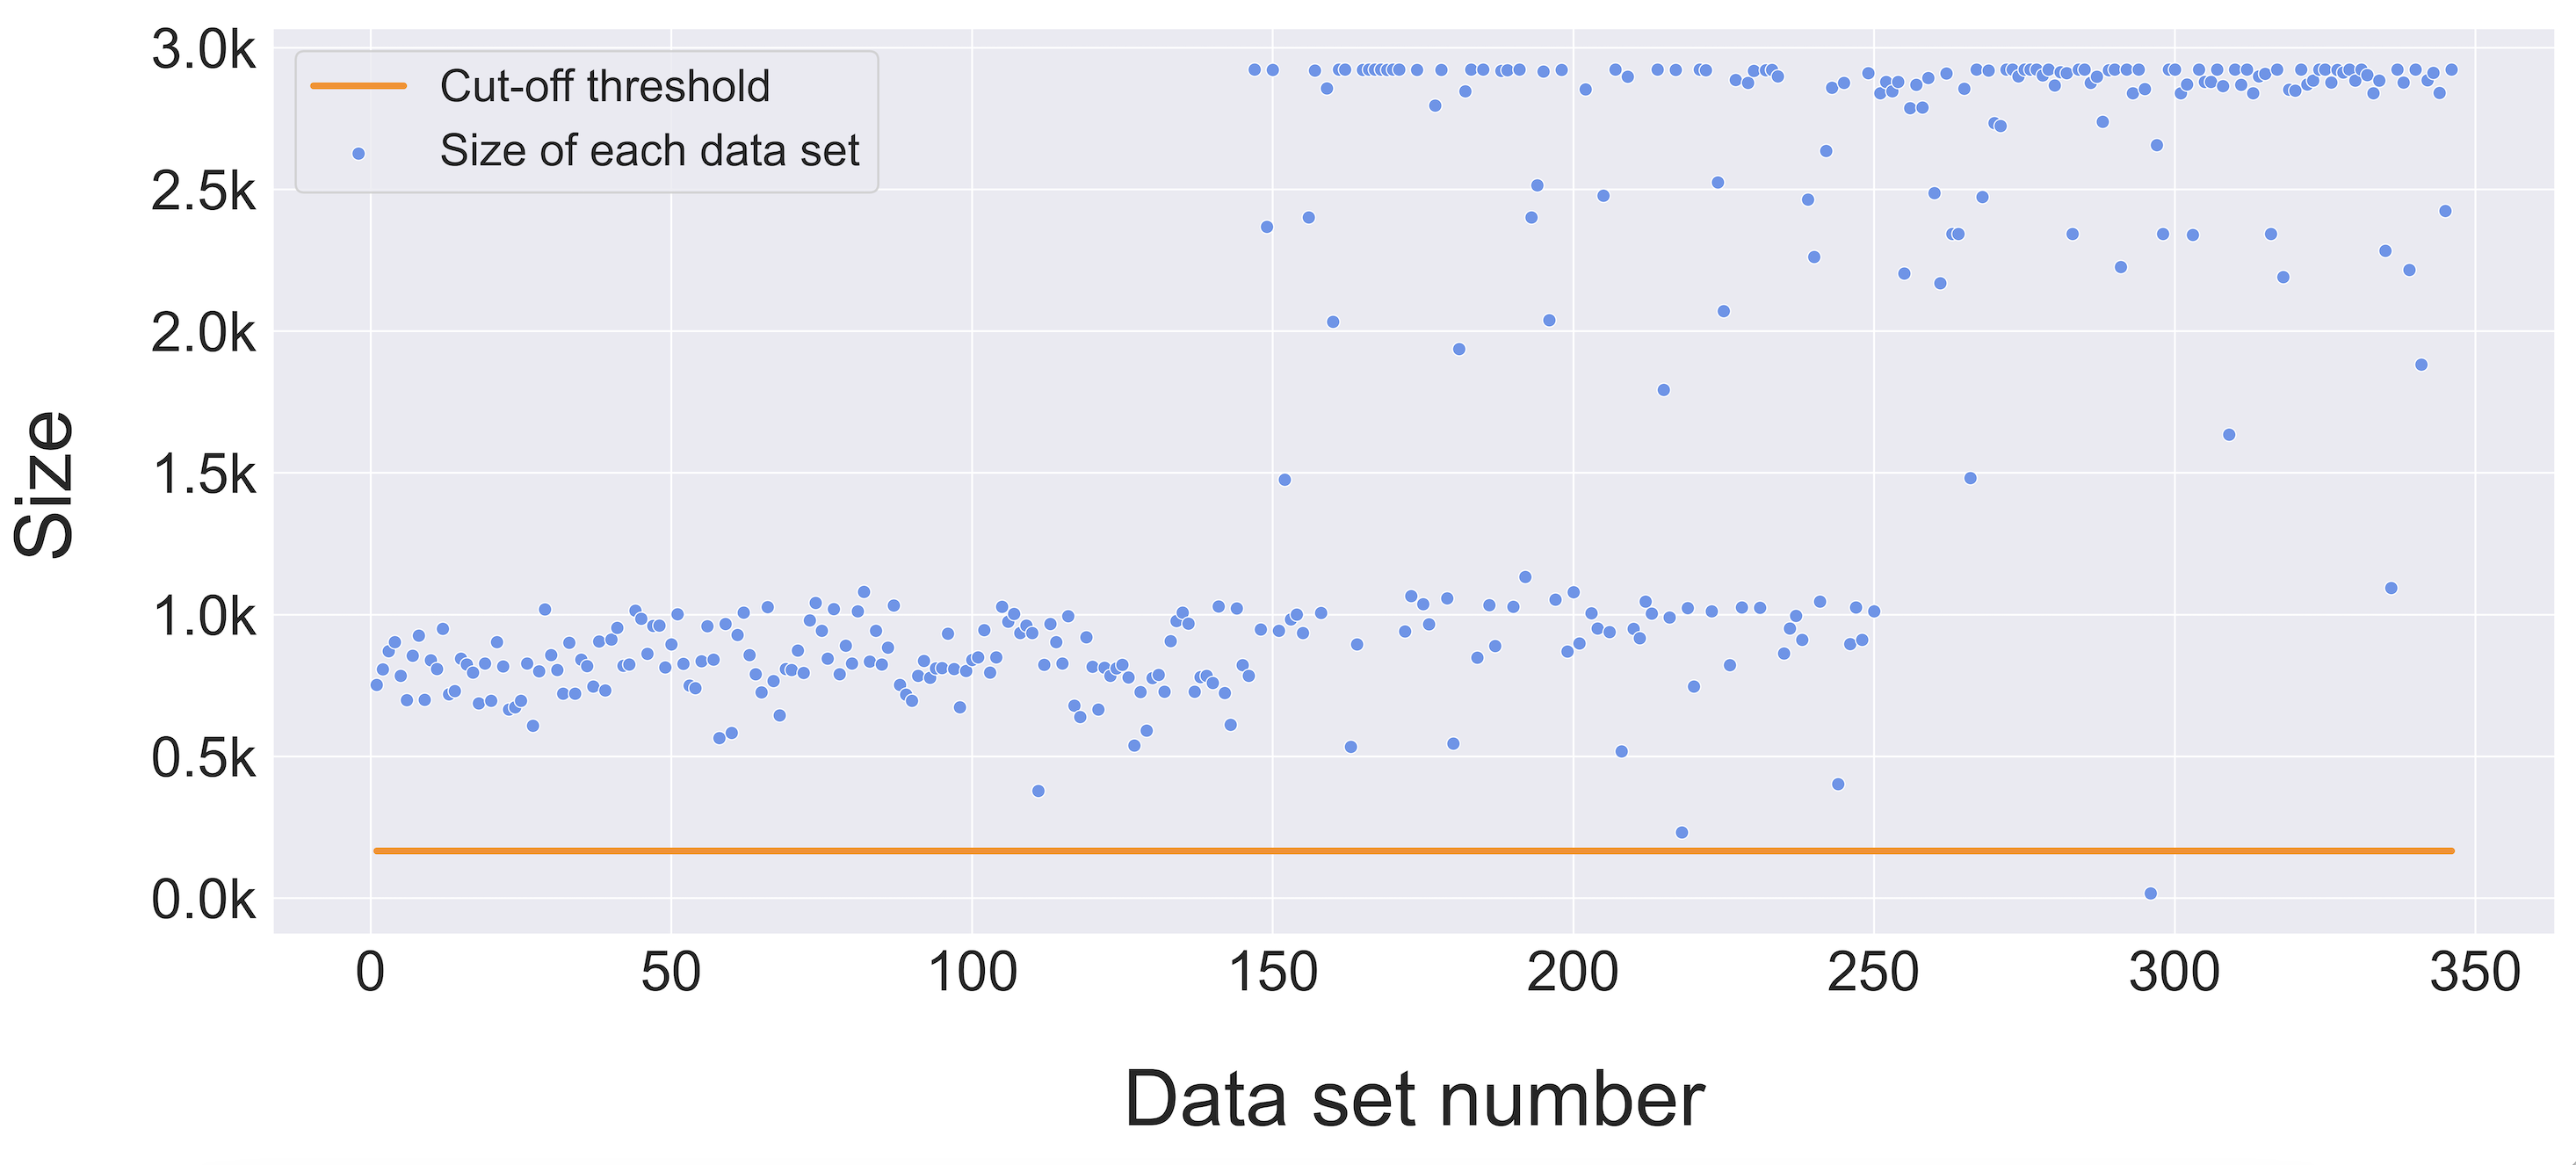
\includegraphics[width=1\textwidth]{Figures/dataset_Y.png}}
  \caption[Data set sizes]{The figures show the data set sizes of X and Y and the proposed cut-off threshold at 10 $\%$ of the mean set size.}
\end{figure}



%%%%%%%%%%%%%%%%%%%%%%%%%%%%%%%%%%%%%%%%%%%%%%%%%%%%%%%%